\documentclass[../main.tex]{subfiles}

\begin{document}

\section{Plasmas en el laboratorio, en la tierra y en el universo}
\lhead[\thepage]{\thesection. Plasmas en el laboratorio, en la tierra y en el universo}

El plasma, en su descripción más básica, consiste en un gás de partículas con carga eléctrica. Los primeros experimentos, que involucraron este estado de la materia, fueron los tubos de descarga de vacío, en los cuales, se producían haces de electrones dentro de un tubo de vidrio y en el cual, se tenían densidades bajas de algún gas. Esto permitía que los electrones, al ser acelerados por alguna fuente de energía, pudiesen ionizar el gas circundante, y formar este sistema complejo de partículas ionizadas. Sin embargo, el primero en usar la palabra "Plasma" fue el físico y químico Irving Langmuir, en su estudio de las oscilaciones en gases ionizados \cite{langmuir1928oscillations}. \\

    \begin{figure}[hbtp]
        %\centering
        \subfigure[]{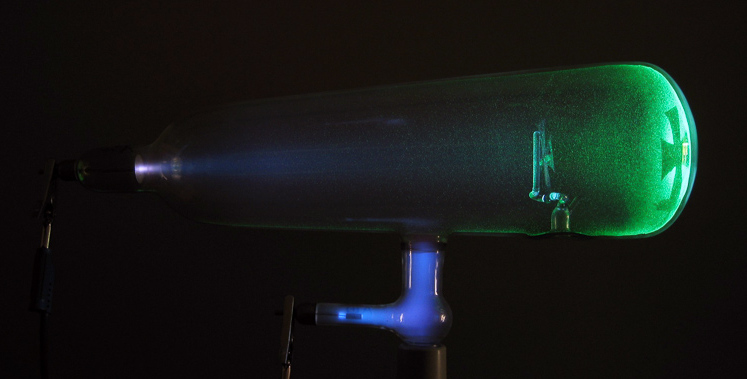
\includegraphics[width=8cm,height=5cm]{Images/Tubo_Crookes.jpeg}}
        \subfigure[]{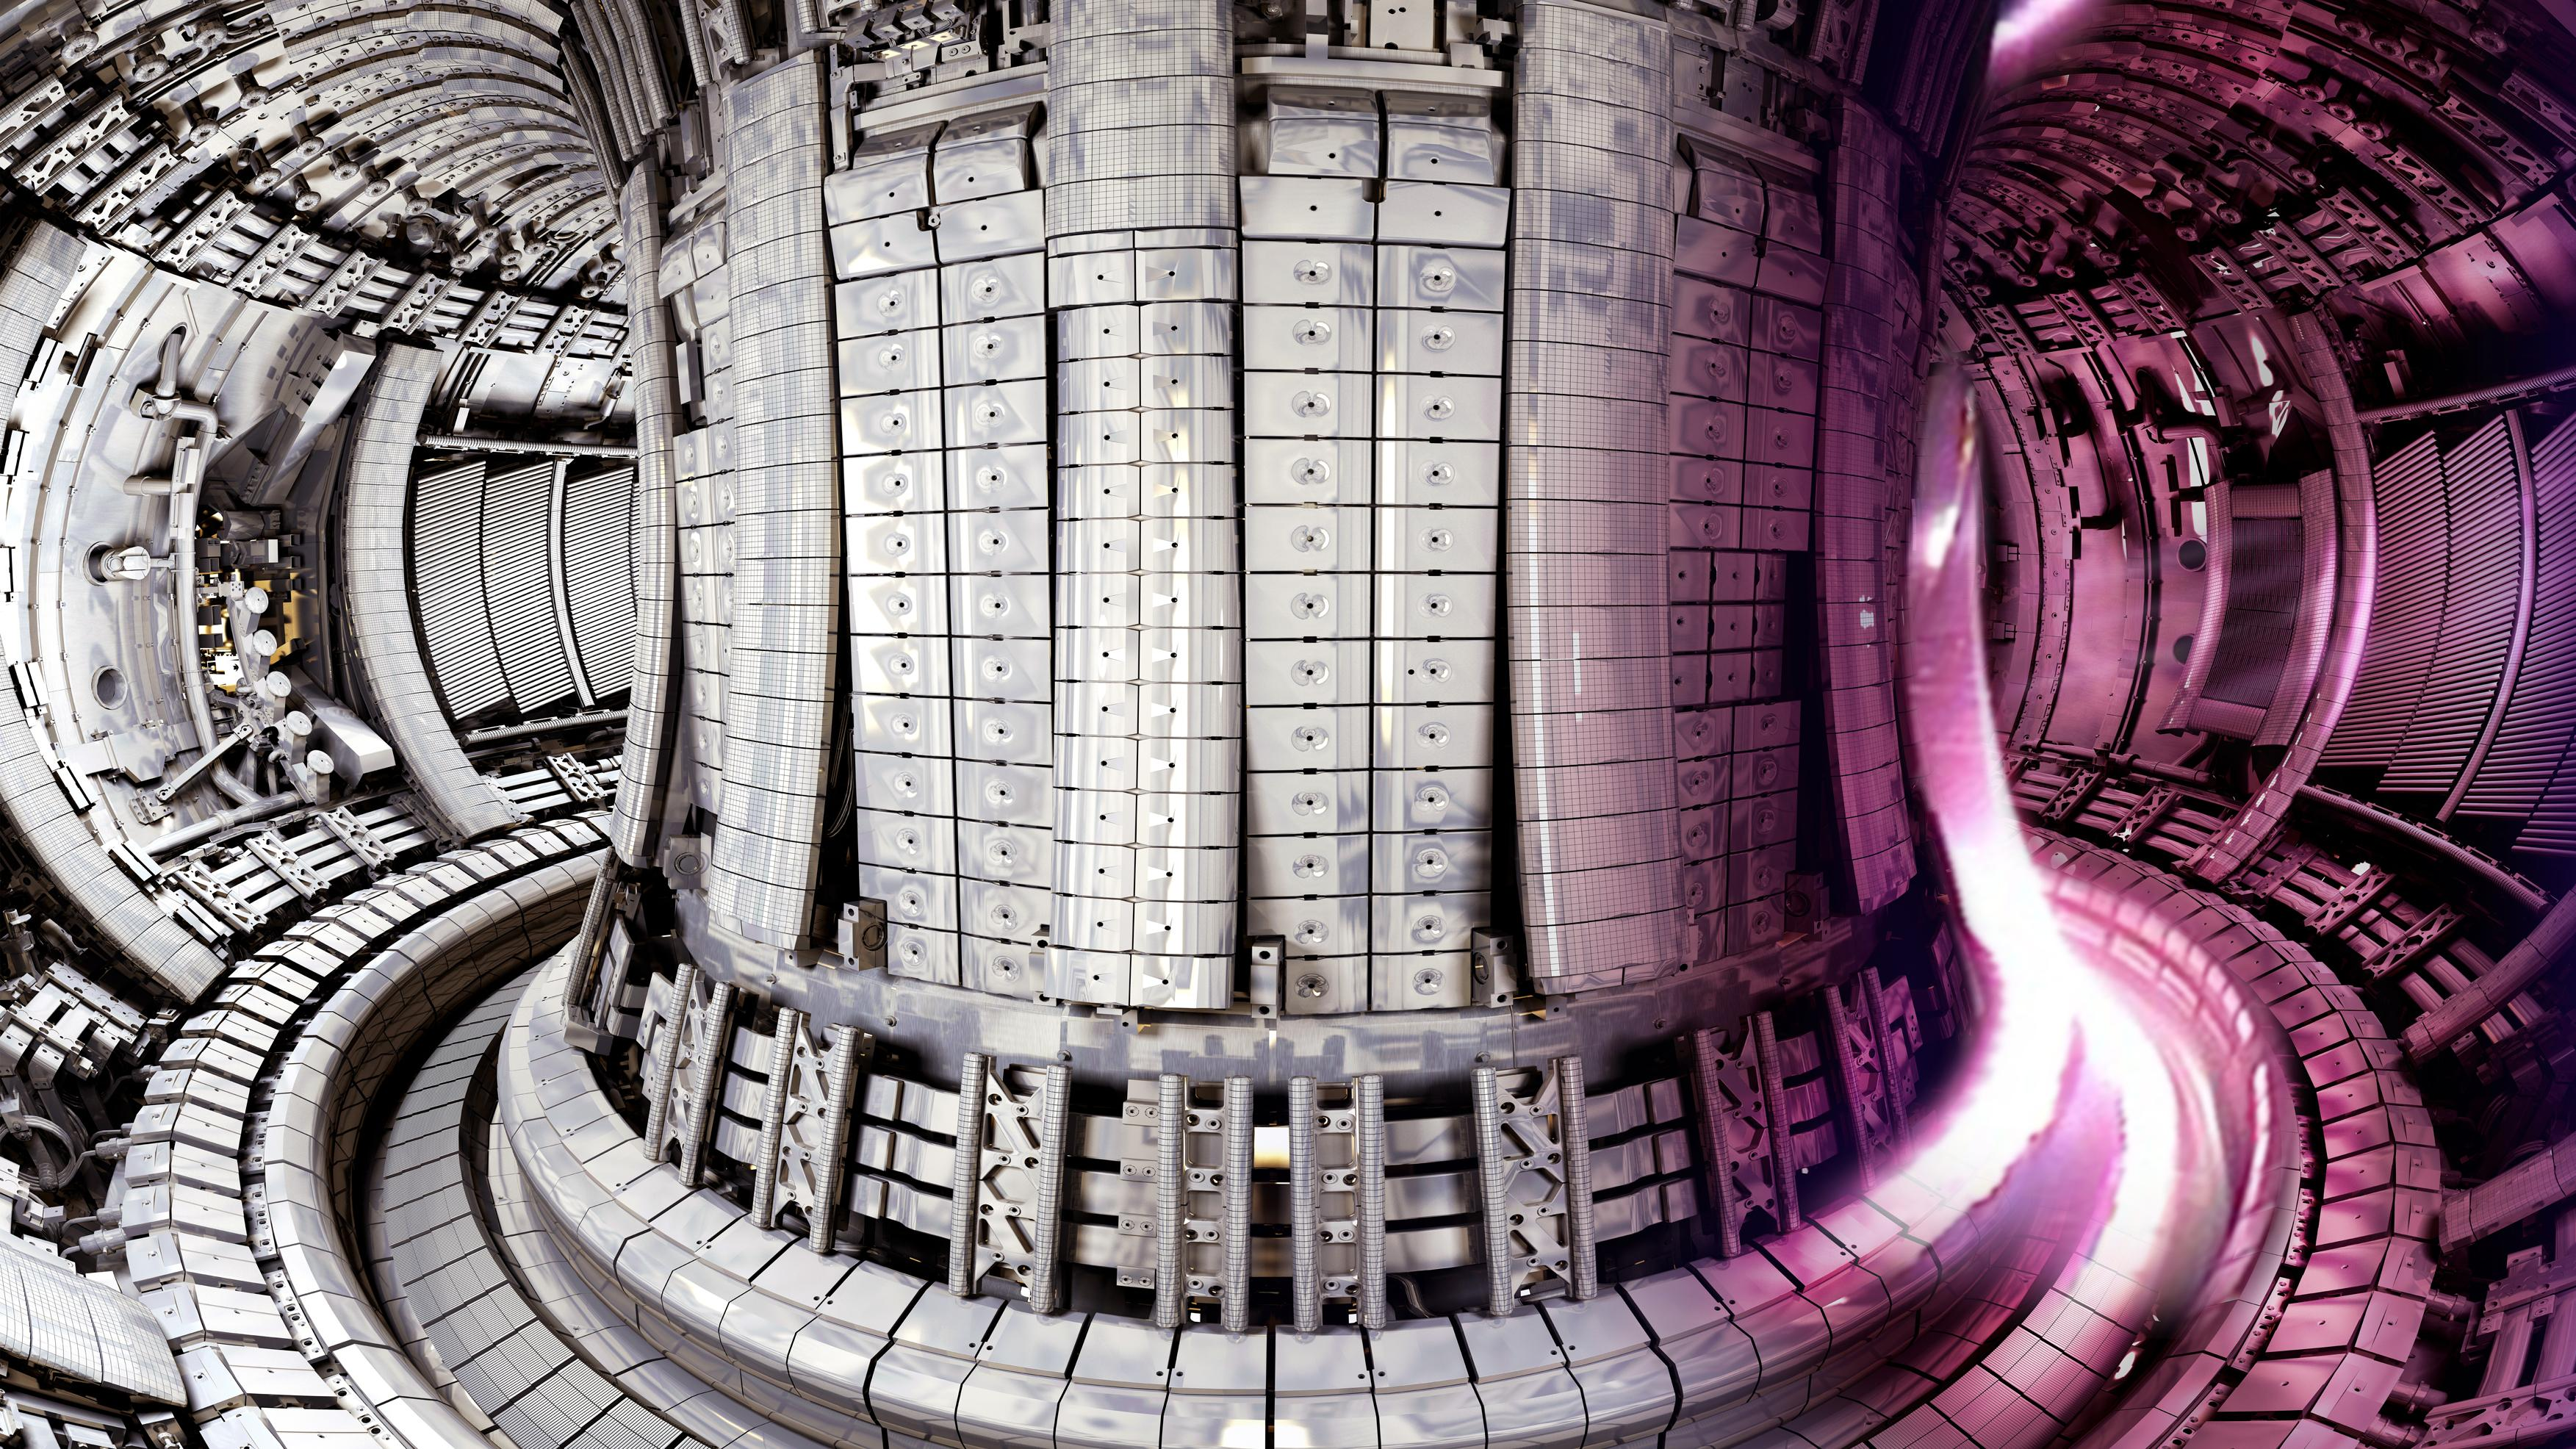
\includegraphics[width=8cm, height=5cm]{Images/JET_Fusion_reactor.jpeg}}
        \caption{a) El tubo de Crookes fue uno de los primeros tubos de descarga de vacío que se utilizo para el estudio de los haces de electrones. b) El JET (Joint uropean Torus) es el reactor de fusión tipo tokamak más grande construido hasta ahora. En su interior, se confinan plasmas a altas temperaturas para que las núcleos atómicos puedan fusionarse. } \label{fig:cap1}
    \end{figure}

%    \begin{figure}[h]
%        \caption{Reactividad de fusión}
%        \centering
%        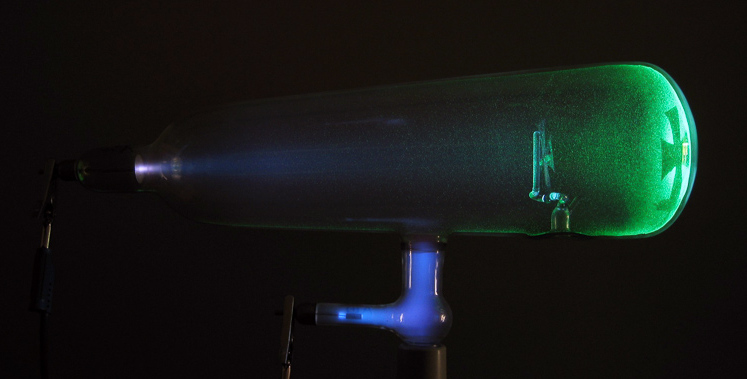
\includegraphics[width=9cm, %height=9cm]{Images/Tubo_Crookes.jpeg}
%    \end{figure}
Los gases ionizados se pueden encontrar en diversos lugares, así como también pueden ser producidos artificialmente. Solo basta proporcionarle cierta energía a un gas neutro para que sus átomos se exciten y se puedan ionizar. Existe una gran variedad de sistemas físicos en este estado, y se pueden clasificar según la densidad de partículas y la temperatura que tengan. Para que un gas ionizado, pueda ser considerado como un plasma, debe manifestar los fenómenos colectivos que se observan en la materia en este estado. El apantallamiento de potenciales eléctricos (Apantallamiento de Debye), dentro de un plasma, sirve como referencia para estudiarlo. Se establece entonces que, para que un plasma exhiba este comportamiento, el número de electrones dentro de una esfera de Debye, debe ser mayor a uno, o
\begin{align}
&N_D = \frac{4}{3}\pi \lambda_D^3 n, \\
&N_D >> 1,
\end{align}
donde $\lambda_D$ es la longitud de apantallamiento de Debye, y su naturaleza y características serán estudiadas en el capítulo 2.
 \begin{figure}[h] 
        \centering
        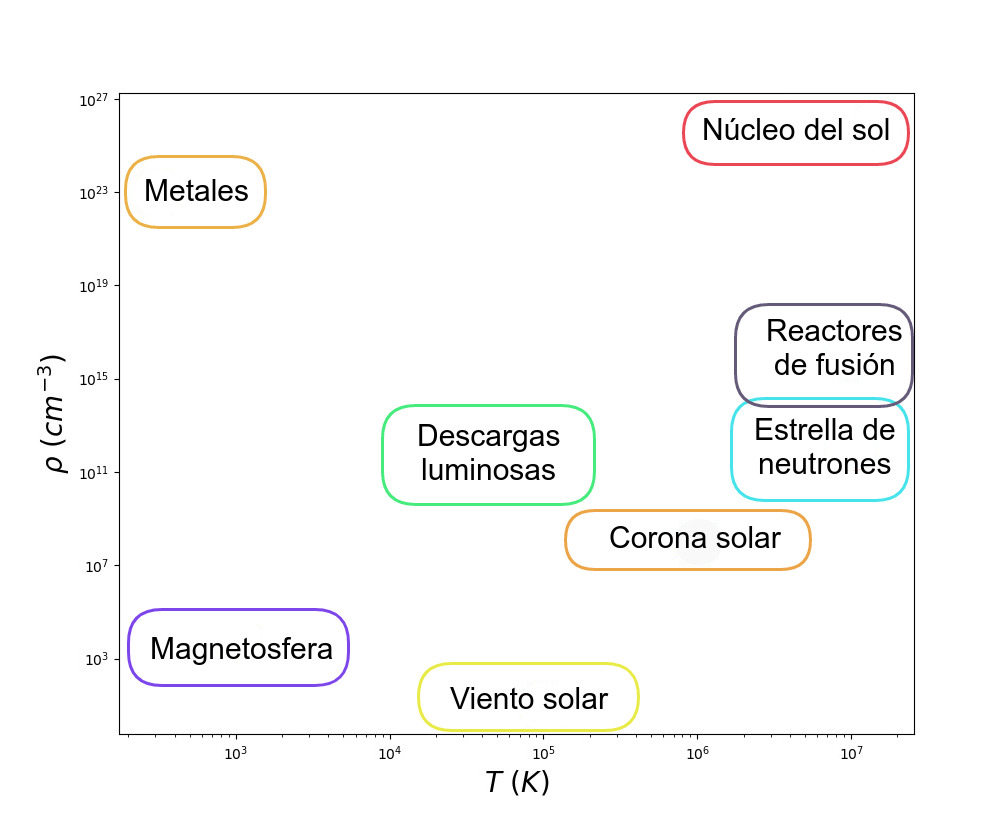
\includegraphics[width=0.8\textwidth]{Images/plasmas_dens_T.jpg}
        \caption{Podemos encontrar plasmas en diferentes lugares del universo, a distintas densidades y temperaturas. Aunque el metal sólido no es un plasma, podemos observar que la densidad de electrones libres es mucho mayor que algunas densidades de plasma.}
        \label{fig:plasmas_dens}
    \end{figure}
    
A nivel de laboratorio, se utilizan campos eléctricos y magnéticos intensos en gases confinados, para estudiar las propiedades del plasma artificial. Actualmente, el plasma tiene muchas aplicaciones en la modificación de las propiedades de superficies en ciertos materiales, como en la electrónica o hasta en la salud. A mayor escala, estos plasmas son utilizados en grandes reactores de fusión, a mayores temperaturas. En la tierra, podemos encontrarlo naturalmente en las capas de la atmósfera, como la ionosfera, debido a la radiación ultravioleta ionizante. Las descargas eléctricas o rayos también producen plasmas, ya que liberan mucha energía y calientan el aire circundante, pues pueden llegar a estar a una temperatura igual a 30 000 K, más de 80 veces la temperatura necesaria para que el agua líquida pase a estado gaseoso. \\

Otros fenómenos que involucran a plasmas son las auroras, cuya manifestación se debe a la interacción del viento solar con la magnetosfera, lo que cambia la dinámica de los iones y electrones, excitando e ionizando la atmósfera superior, y produciendo esos característicos colores verde. Más allá de la tierra, tenemos los espacios interplanetarios e interestelares, que también están conformados por gases ionizados a cierta densidad. Sin embargo, también encontramos lugares donde el plasma juega un papel importante en el universo, y en la vida misma aquí en la tierra. Las estrellas como nuestro sol, concentran plasmas a altísimas temperaturas y presiones, para poder fusionar los núcleos o iones, y liberar grandes cantidades de energía. Así es como pueden brillar, y gracias a esto es que, la tierra puede tener una atmósfera equilibrada para la vida. Otros lugares son las nebulosas, que son los restos de una explosión de una estrella masiva. Vemos entonces que, el plasma puede existir en un gran rango de magnitud, en densidad y temperatura, como se ve en la Figura (\ref{fig:plasmas_dens}). 

\section{Fenómenos físicos en un plasma: Condición de Bohm}
\lhead[\thepage]{\thesection. Fenómenos físicos en un plasma: Condición de Bohm}

Debido a la complejidad de las interacciones dentro del plasma, se puede describir una gran variedad de fenómenos dentro del mismo. Procesos difusivos, debidos al gradiente de densidades de las partículas en el sistema, o procesos disipativos, en los cuales se ven los mecanismos de perdida de energía, ya sea por colisiones dentro del plasma sin una inyección adicional de energía, o por la radiación emitida por las partículas cargadas, debido a su aceleración o curvatura en sus trayectorias (radiación de sincrotrón). También encontramos fenómenos con carácter ondulatorio, como los provocados por pequeñas perturbaciones en las densidades, o desplazamientos de carga.
\begin{figure}[htbp]
        \centering
        \subfigure[]{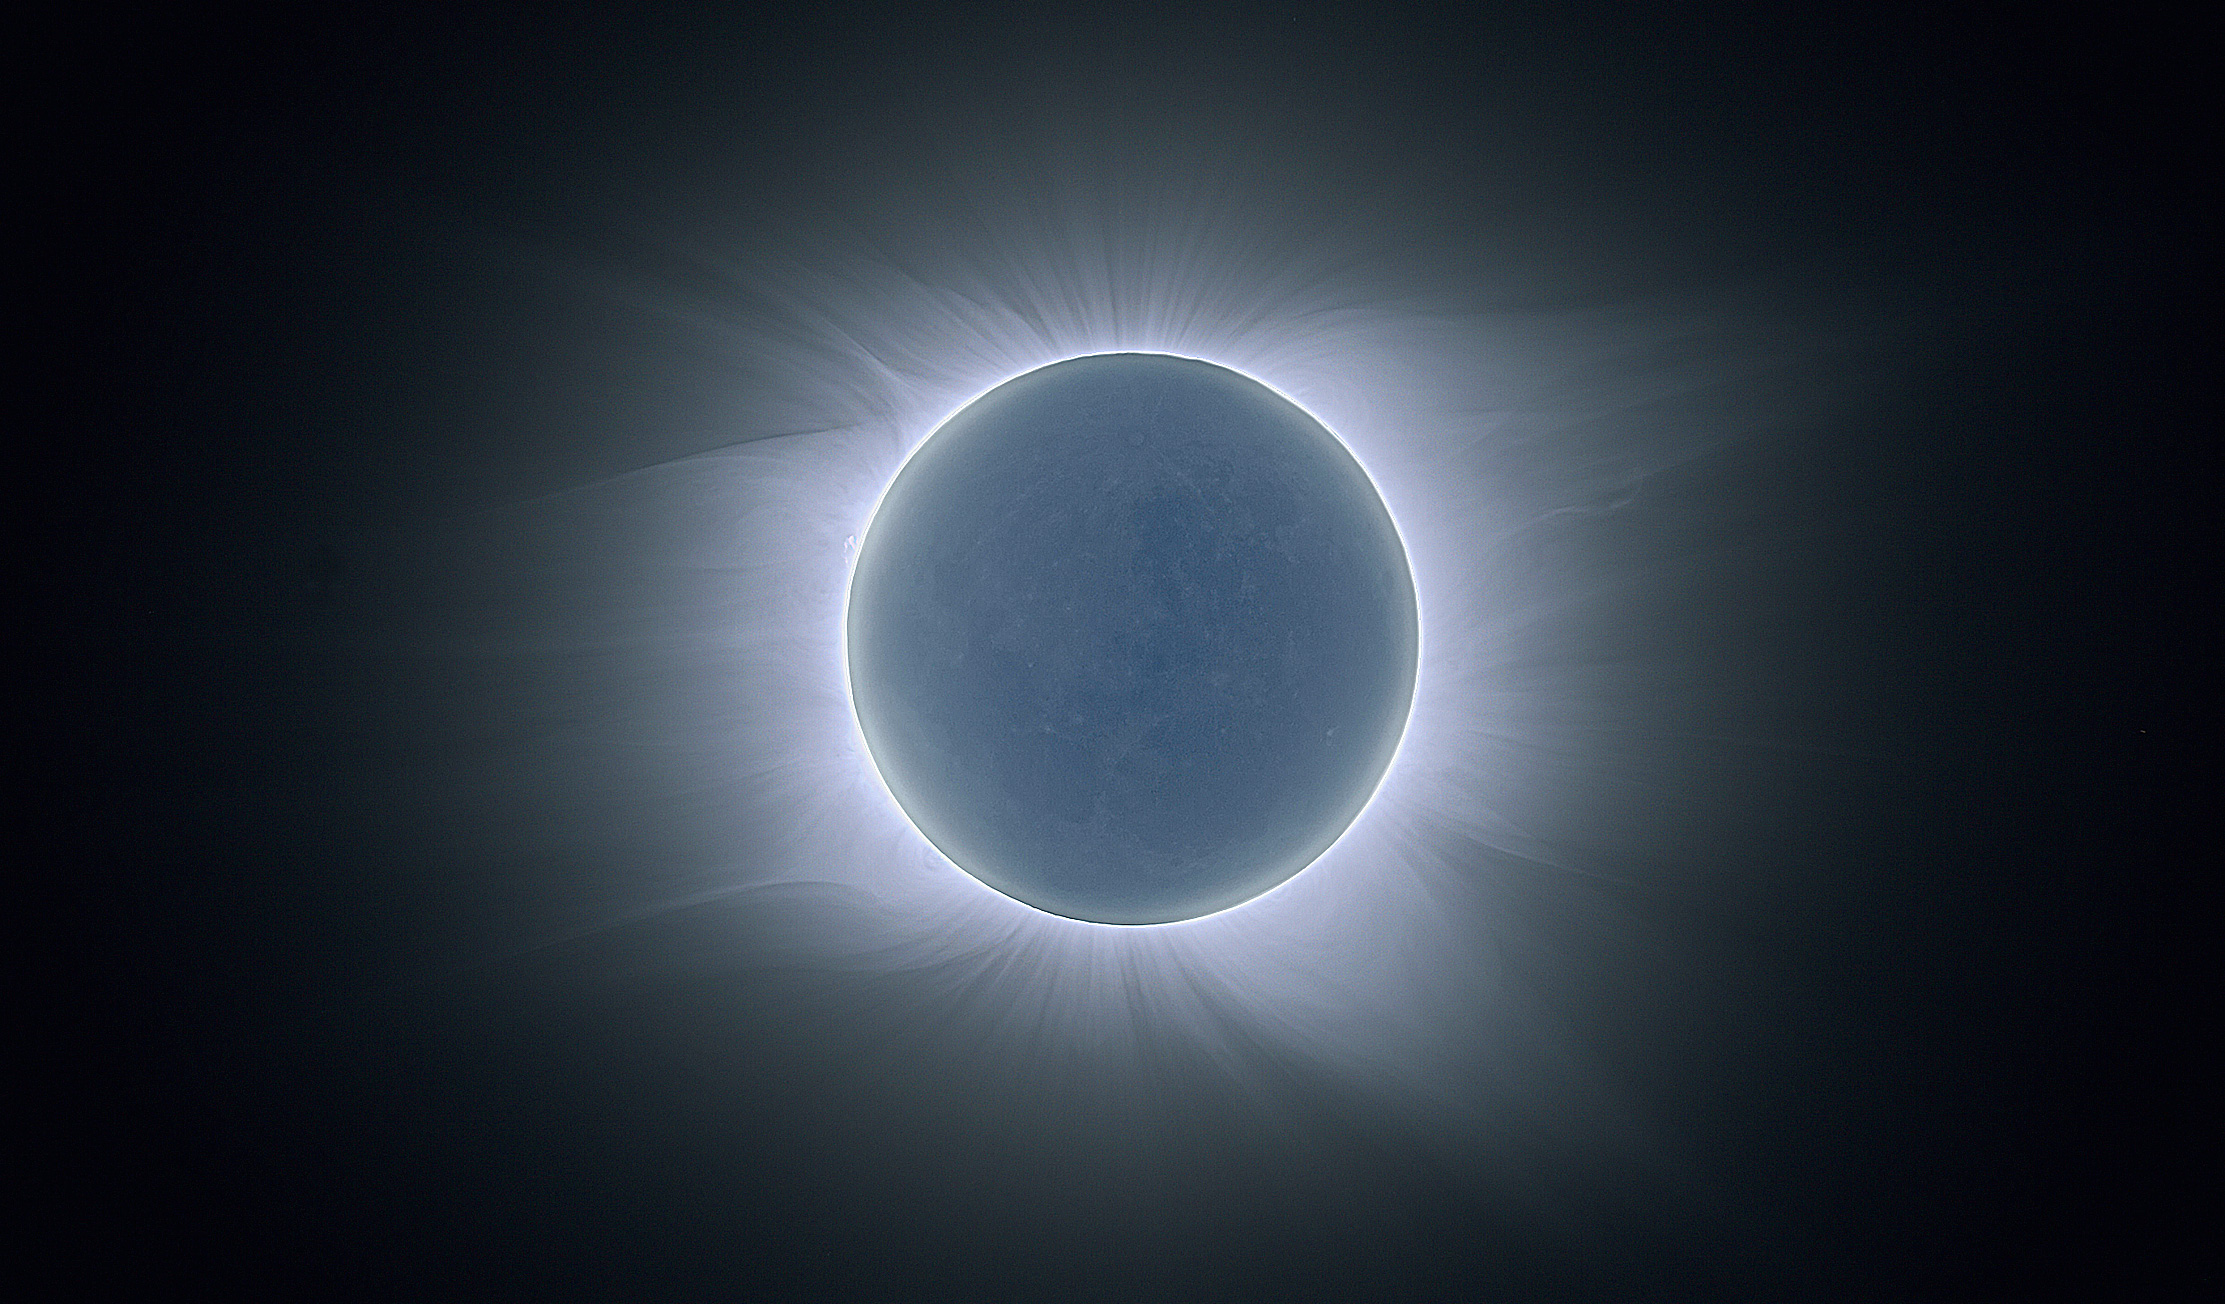
\includegraphics[width=7cm, height=4cm]{Images/corona_solar.jpeg}}
        \subfigure[]{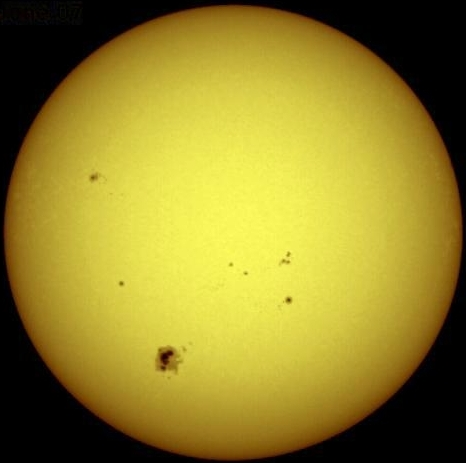
\includegraphics[width=4cm, height=4cm]{Images/fotosfera.jpeg}}
        \caption{Los fenómenos ondulatorios en el plasma son muy estudiados en la dinámica del sol. La corona solar (a), y la fotósfera (b), son dos regiones a temperaturas muy distintas, ya que la primera, al ser una capa superior se encuentra a mayor a temperatura que la segunda. Se cree que las ondas de Alfvén, que son perturbaciones que transportan energía a lo largo de campos magnéticos, podrían explicar esto.} \label{fig:cap1}
    \end{figure}

Esto provoca que el plasma, en un inicio, oscile localmente a una determinada frecuencia, denominada frecuencia del plasma, y que posteriormente, el campo eléctrico resultante de esta oscilación, afecte a capaz subyacentes en el plasma, y se tengan oscilaciones que se propaguen dentro del sistema. Aunque el espectro de estudio del plasma es muy amplio, una parte de el se enfoca en aquellos que son usados en procesos de fusión nuclear, o llamados también plasmas termonucleares. Estos plasmas son manipulados a través de campos magnéticos que influyen en el movimiento de las partículas, conteniéndolos dentro de un reactor para que los núcleos (iones) adquieran suficiente energía y proximidad entre ellos, para fusionarse. \\

    
El correcto comportamiento del plasma dentro de un reactor, para los fines perseguidos, es objeto de gran estudio e investigación. Una de parte de ello, se encarga de la interacción plasma-pared. Como ya se mencionó, un reactor utiliza potentes campos magnéticos para confinar el movimiento de las partículas cargadas. Sin embargo, este confinamiento no es perfecto, y siempre se tiene cierta cantidad de partículas que escapan del sistema. En un modelo simplificado, que consta de un gas de partículas a cierta densidad y temperatura de equilibrio $n$ y $T$, dentro de un recipiente con paredes metálicas, y en donde no se tiene la influencia de algún campo magnético, las partículas cargadas tenderán a acumularse sobre las paredes, producto de su movimiento aleatorio. Esta acumulación no es igual para cada especie de partícula, debido a que, por lo general, se tiene diferentes equilibrios ($T$) para cada especie. Además, es importante considerar la relación de masa entre las partículas, ya que para un electrón y un protón solamente, está relación es de aproximadamente $1/1868$. Esta diferencia hará que la inercia de los electrones sea mucho menor que la de los iones, y por la tanto, facilitará el movimiento de los mismos. Los electrones comenzarán a acumularse más rápido que los iones, lo que provocará la aparición de un potencial negativo, que repele a los electrones y atrae  a los iones, y el flujo de incidencia comenzará a igualarse para ambas especies. En el equilibrio, se formará una delgada capa o "funda'' en la pared del contenedor, en la que la densidad de electrones es menor que la de los iones. Este potencial de pared se filtrará mínimamente dentro del plasma, pero lo suficiente como para, en cierta región, acelerar a los iones hasta velocidades sónicas antes de ingresar a la zona de baja densidad electrónica. Está comportamiento dinámico por parte de los iones es conocido como condición de Bohm, el cuál será estudiado en el capítulo 5. \\

\begin{figure}[h] 
        \label{fig:figura2.1}
        \centering
        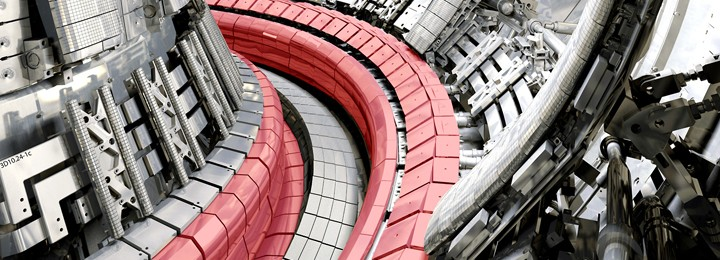
\includegraphics[width=0.8\textwidth]{Images/divertor_jet.jpg}
        \caption{La regiones de color rojo, son las zonas específicas donde el plasma entrará en contacto con el tokamak. En la imagen, se puede observar la configuración denominada Divertor, en el reactor de fusión JET. }
\end{figure}
\newpage
\section{Fusión Nuclear, como alternativa energética}
\lhead[\thepage]{\thesection. Fusión Nuclear, como alternativa energética}
Es un hecho que la humanidad no podrá sostener su consumo energético por mucho tiempo, si es que las principales fuentes de energía siguen proveniendo de recursos no renovables, como el petróleo o el carbón. Por otra parte, el impacto ambiental negativo que tienen es muy alto. Esto lo podemos ver claramente en la centrales de fisión nuclear, en donde los riesgos de la exposición a la alta radiación siempre han sido preocupantes, y un escenario que siempre debe considerarse. Por esta razón, es indispensable poder contar con fuentes energéticas de mayor alcance y seguridad. Las energías renovables, como la eólica o solar, son algunas opciones que ya se están utilizando y a la vez, desarrollando, pero que aún necesitan ocupar mucho espacio para satisfacer la demanda eléctrica actual. La fusión nuclear es tal vez, la más prometedora de esas, aunque muy esquiva actualmente. La fusión nuclear, es un fenómeno físico en el que dos núcleos atómicos se fusionan, y como resultado de esta reacción se liberán otras partículas, tales como neutrones y otros núcleos más pesados. La reacción puede ser descrita como
    \begin{align}
        X + Y \rightarrow Z + n,
    \end{align}
en donde $X$ e $Y$ son los núcleos ligeros que reaccionarán, mientras que $Z$ y $n$ son el núcleo pesado resultante, y la partícula energética, tal como el neutrón, respectivamente. El balance energético se determina por medio de la relación masa-energía de A. Einstein
    \begin{align}
        E = mc^2.
    \end{align}

La energía liberada, por ejemplo, en una reaccion de fusion D-T (deuterio-tritio) es igual a 17.6 MeV. Para una reacción de fisión de U-235, la energía promedio liberada por núcleo dividido es de 200 Mev. Si comparamos ambas cantidades, podemos observar que la energía liberada
por reacción, es aproximadamente 11 veces mayor en la fisión de núcleos que en la fusión. Sin embargo, si consideramos grandes cantidades de material reactivo, esta diferencia energética se vuelve favorable para las reacciones de fusión, debido a que se tienen mas moles de D-T por kilogramo, que moles de U-235. Además, el deuterio es un isótopo abundante del hidrógeno, y el tritio puede ser obtenido a travez del litio por bombardeo de neutrones. El uranio, por otro lado, es más escaso y se encuentra naturalmente formado por tres tipos de isotopos, en donde el U-235 solo representa el 0.71\% por gramo, por lo que para una reacción de fisión exitosa, se debe tener cierto grado elevado de pureza, lo cual es difícil de lograr.\\

Además, una reacción de fisión puede desencadenar muchas otras más, y si estás no son controladas, puede conducir a catastrofes medioambientales enormes, debido al material radiactivo que puede ser liberado hacia el exterior y afectar gravemente a los seres vivos alrededor. En la fusión, por el contrario, lo que se busca es mantener el número de reacciones, y si esto no se logra, el proceso se apaga a sí mismo. Aunque el riesgo de producir materiales radiactivos debido al desprendiemiento de neutrones en la fusión nuclear también está presente. Actualmente, la fisión nuclear nos da un soporte energético considerable. La tecnología actual y los protocolos de seguridad permiten aprovechar este fenómeno físico satisfactoriamente, aunque cualquier mínimo error conllevaría consecuencias enormes. Por otro lado, la fusión nuclear aún se encuentra en fase de desarrollo y experimentación, pero actualmente ya se han dado pasos enormes en la fabricación de reactores y tecnologías involucradas. Uno de estos, ITER (International Thermonuclear Experimental Reactor), planea ser el proyecto de fusión más grande de la década. Su culminación permitirá estudiar a mayores escalas muchos aspectos de este fenómeno en un ambiente controlado, tanto en la parte teórica como técnica, y servir como evidencia de que la energía de fusión será la energía del futuro. \\

\begin{figure}[h] 
        \label{fig:figura2.1}
        \centering
        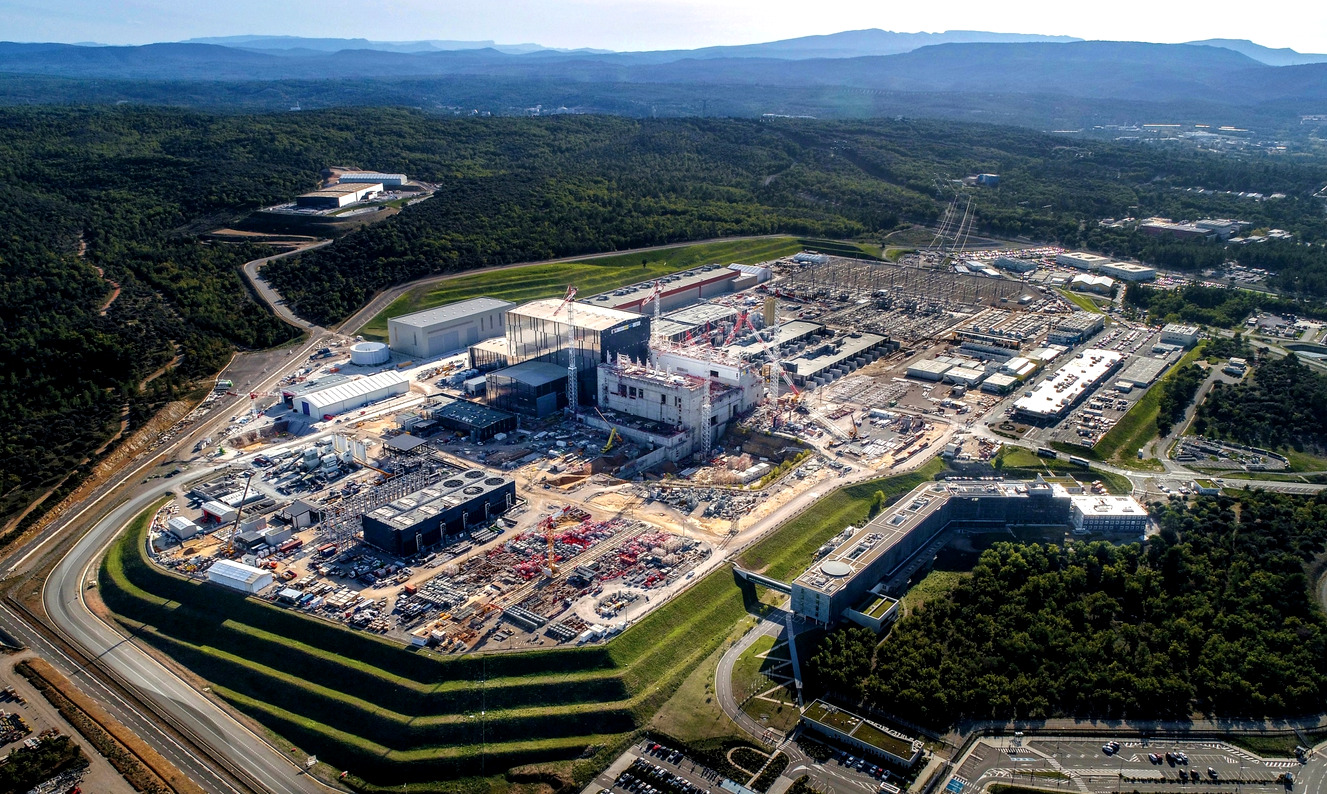
\includegraphics[width=0.8\textwidth]{Images/ITER.jpg}
        \caption{ITER, ubicado en Cadarache, al sur de Francia, será un reactor de fusión experimental capaz de producir 10 veces la potencia suministrada. Aunque no está previsto que funcione como una planta de energía de fusión nuclear, permitirá asentar el camino para DEMO (DEMOnstration Power Plant), el que se piensa será el primer prototipo de reactor de fusión nuclear comercial.}
\end{figure}

\begin{comment}

Por lo que al determinar la energía total inicial y final, considerando solo las masas de los núcleos, tendremos que parte de la energía inicial se encuentra en forma de energía cinética en las partículas finales. Esta energía puede ser utilizada para, por ejemplo, calentar agua y generar vapor, que mueva una turbina y producir corriente eléctrica. Por esta razón, este fenómeno es considerado como alternativa para la producción de energía aprovechable. Sin embargo, muchas cuestiones de estudio, tanto en la parte teórica como técnica, hacen que esto sea un gran desafío para la época actual. 

\end{comment}
 


\end{document}